In order to evaluate the consistency and the reliability of our application we have conducted some unit tests. \\
The tests regard the business logic tier, the core of the application in terms of complexity and relevance of computation.\\
Considering that the business logic classes interacts directly with data in the database, we had to adopt a specific framework, named "Mockito" to Mock the method calls which retrieve data from the database and to specify an action to be performed in case of calls during testing execution.\\
It is relevant to say that we adopted this mocking framework assuming that the operations related to reading and writing data in the database are executed correctly, indeed they are not tested with a proper testing component. However, we are quite confident that this assumption is consistent because we checked it informally .\\
As far as the unit test are concerned, we have checked them using jUnit libraries.\\
Finally, we have tested also that the calls to the Google Maps APIs,in particular the Distance Matrix API. We checked that it was executed correctly and that the  retrieved information was consistent.\\ 
Further details about the test cases and the related outcomes have been included in the document.\\

\subsection{JUnit and Mockito}


\subsubsection{Meeting vs. Meeting Conflict}
This test case has the purpose to evaluate the method to check whether two meeting are in conflict. Considering that this kind of evaluation involves two meetings at a time, we have  built two meetings, we have assigned them overlapping schedules and we have tested the execution of the method 'CheckMeetingOverlaps(Meeting m)' of the class ConflictCheckerBean.java . The result of the test was consistent with the expected outcome. 

\subsubsection{Meeting vs. Break Conflict}
This test case was made to check whether the conflict among meetings and breaks was computed correctly. Due to the fact that the comparison involves one meeting and one break at a time, we have built a break and a meeting that should have been overlapping and we tested the execution of the method 'BreakConflictChecker(Meeting m)' of the class ConflictCheckerBean.java . As we expectd, the outcome certified that the conflict was computed. 

\subsubsection{Flexible break rescheduling}
In order to verify the flexible break rescheduling, one of the main functions of Travlendar+, we made an apposite test case. This analysis simply consists in calling the method checkReschedule(String uid) of the class ConflictCheckerBean.java and checking that the outcome, in case the flexible rescheduling is infeasible, reports that effectively the meeting and the break are in conflict. 

\subsubsection{Warning existence }
this test case regards this specific situation: a new Meeting is inserted in the db and according to its conflicts, it should be added in an already existent warning in the database.  Hence, this analysis tests whether the already existent warning to be updated is retrieved correctly. To perform the test we have simulated the insertion of a warning in the database and we have created a meeting that had to be added to the existent warning. Then, we have called the method 'checkWarningExistence()' of the class ConflictCheckerBean.java and we verified that the outcome was consistent. 
Finally, for completeness, we replayed the test to check also a situation in which a new warning has to be created. 

\subsubsection{Retrieve duration}
The current test case has the purpose to verify the interaction between our application and the Google Maps APIs. In particular we checked that the requested information is retrieved correctly by testing if the duration of a specific travel is correct, doing this we also tested the connection with Google servers and the correctness of our queries. 
In other words we called the method retrieveDuration(String origin,String destination, String uid, Date date)  of the class RouteCalculatorBean().java and we passed them an origin and a destination parameter for which we already know the travel duration and we expected the same outcome. 

\clearpage
\subsection{JMeter}

We also made a really trivial test to evaluate the non-functional requirements and in particular the performances given an high number of clients requesting a resource. The test was done using JMeter and the simple test consisted having a thousand users trying to access the application by performing a login and visiting the homepage, the requested are done almost all at the same time (ramp-up period equal to zero which means no delay between requests).
\\As you can see from the below graph the latest visited the homepage after less than 3 seconds, which suggests than the performances of the server are already a bit stressed and if the same amount of users requested a more sophisticated resource that would require computationally onerous algorithms by the server, the amount of time requires would probably not be reasonable for a user experience point of view. Notice however that, in such an application, users would mostly navigate in a burstly way, which implies that in order to have a thousand requests at the same exact time, the number of users would have to be much larger than a thousand.

\begin{figure} 
\begin{center}

\makebox[\textwidth]{%
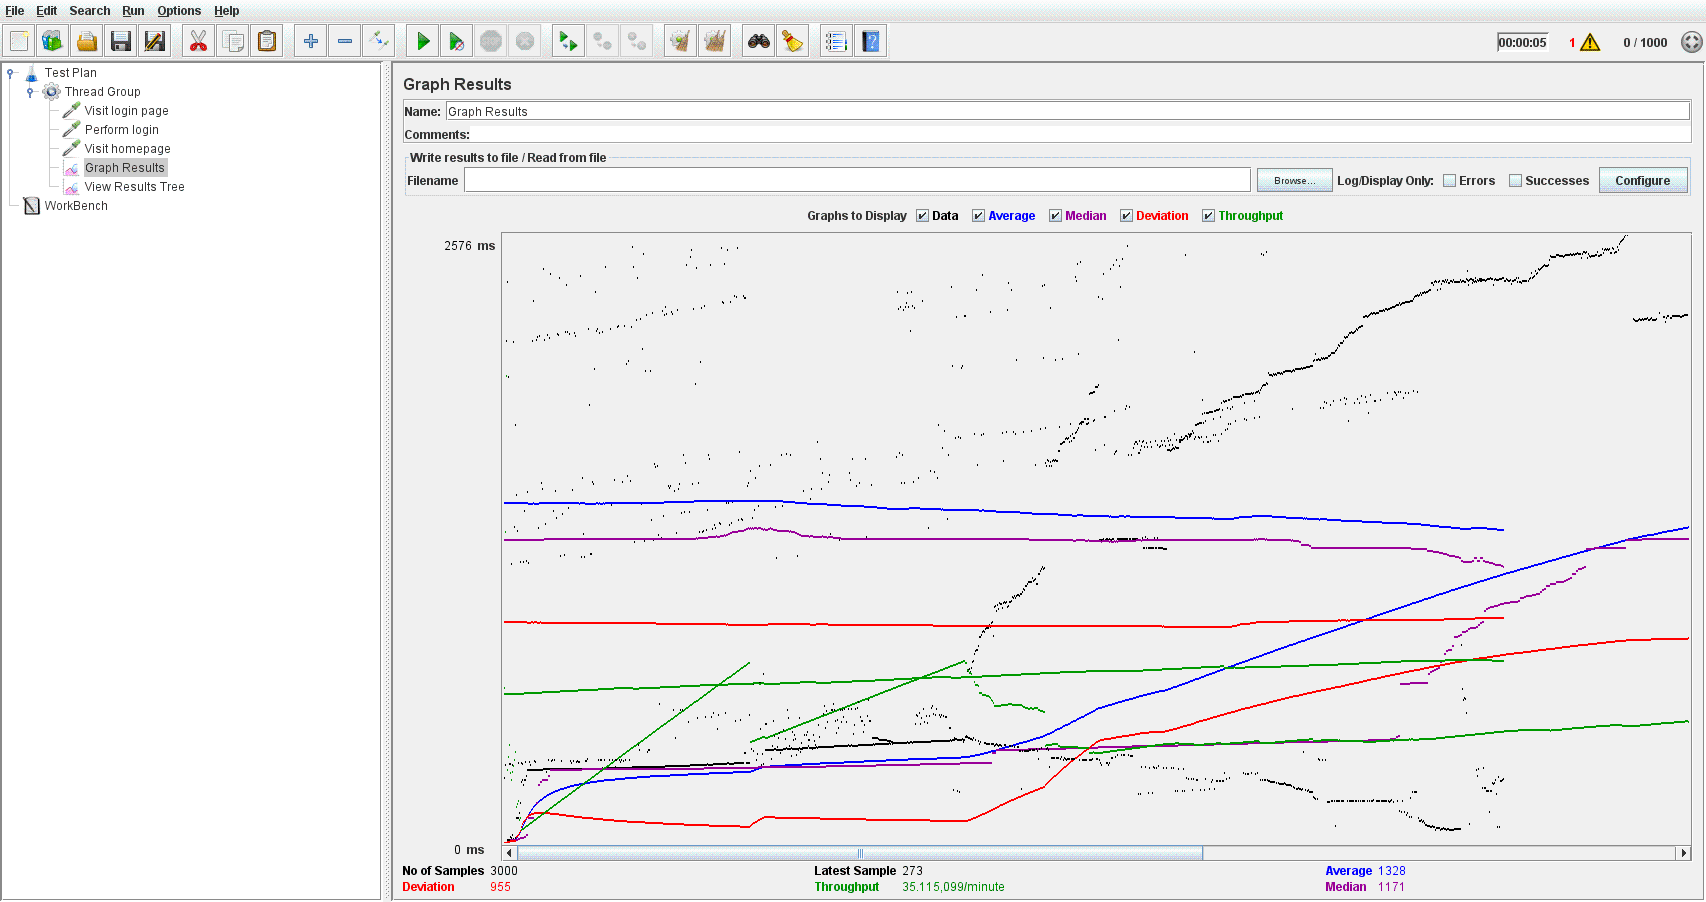
\includegraphics[width=1.5\linewidth]{images/jmeterlogins} 
}
\caption{Graph results of 1000 users that simultaneously try to login} 
\label{fig:jmetertest} 


\end{center}
\end{figure} 


